\section{Background Concepts}
\label{background}

\subsection{United Nations Security Council (UNSC) Corpus}
As the UNSC corpus was already briefly described in the introduction, we will proceed to describe some key statistics regarding this corpus. As mentioned, this corpus contains textual data from 65,393 speeches which were collected from 1995-2017. In Figure \ref{UNSC_stats_1}, we can observe how the number of speeches and meetings vary temporally. We can, for example, notice how there was a peak in the number of speeches per meeting in 2003; which corresponds to the onset of the Iraq war.

\begin{figure}[H]
    \centering
    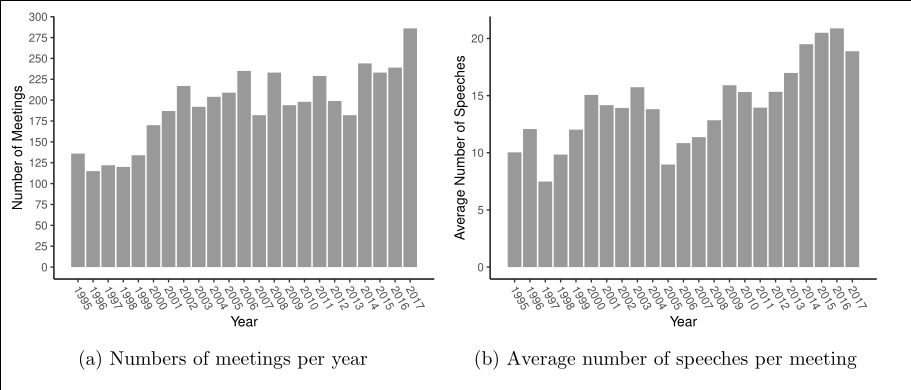
\includegraphics[trim={0.2cm 0.1cm 0 0.1cm},clip,width=\textwidth]{unsc_speeches_stats_1.png}
    \caption{Temporal distribution of the number of speeches and meetings in the UNSC corpus \citep{schnfeld2019security}}
    \label{UNSC_stats_1}
\end{figure}

\begin{figure}[t]
    \centering
    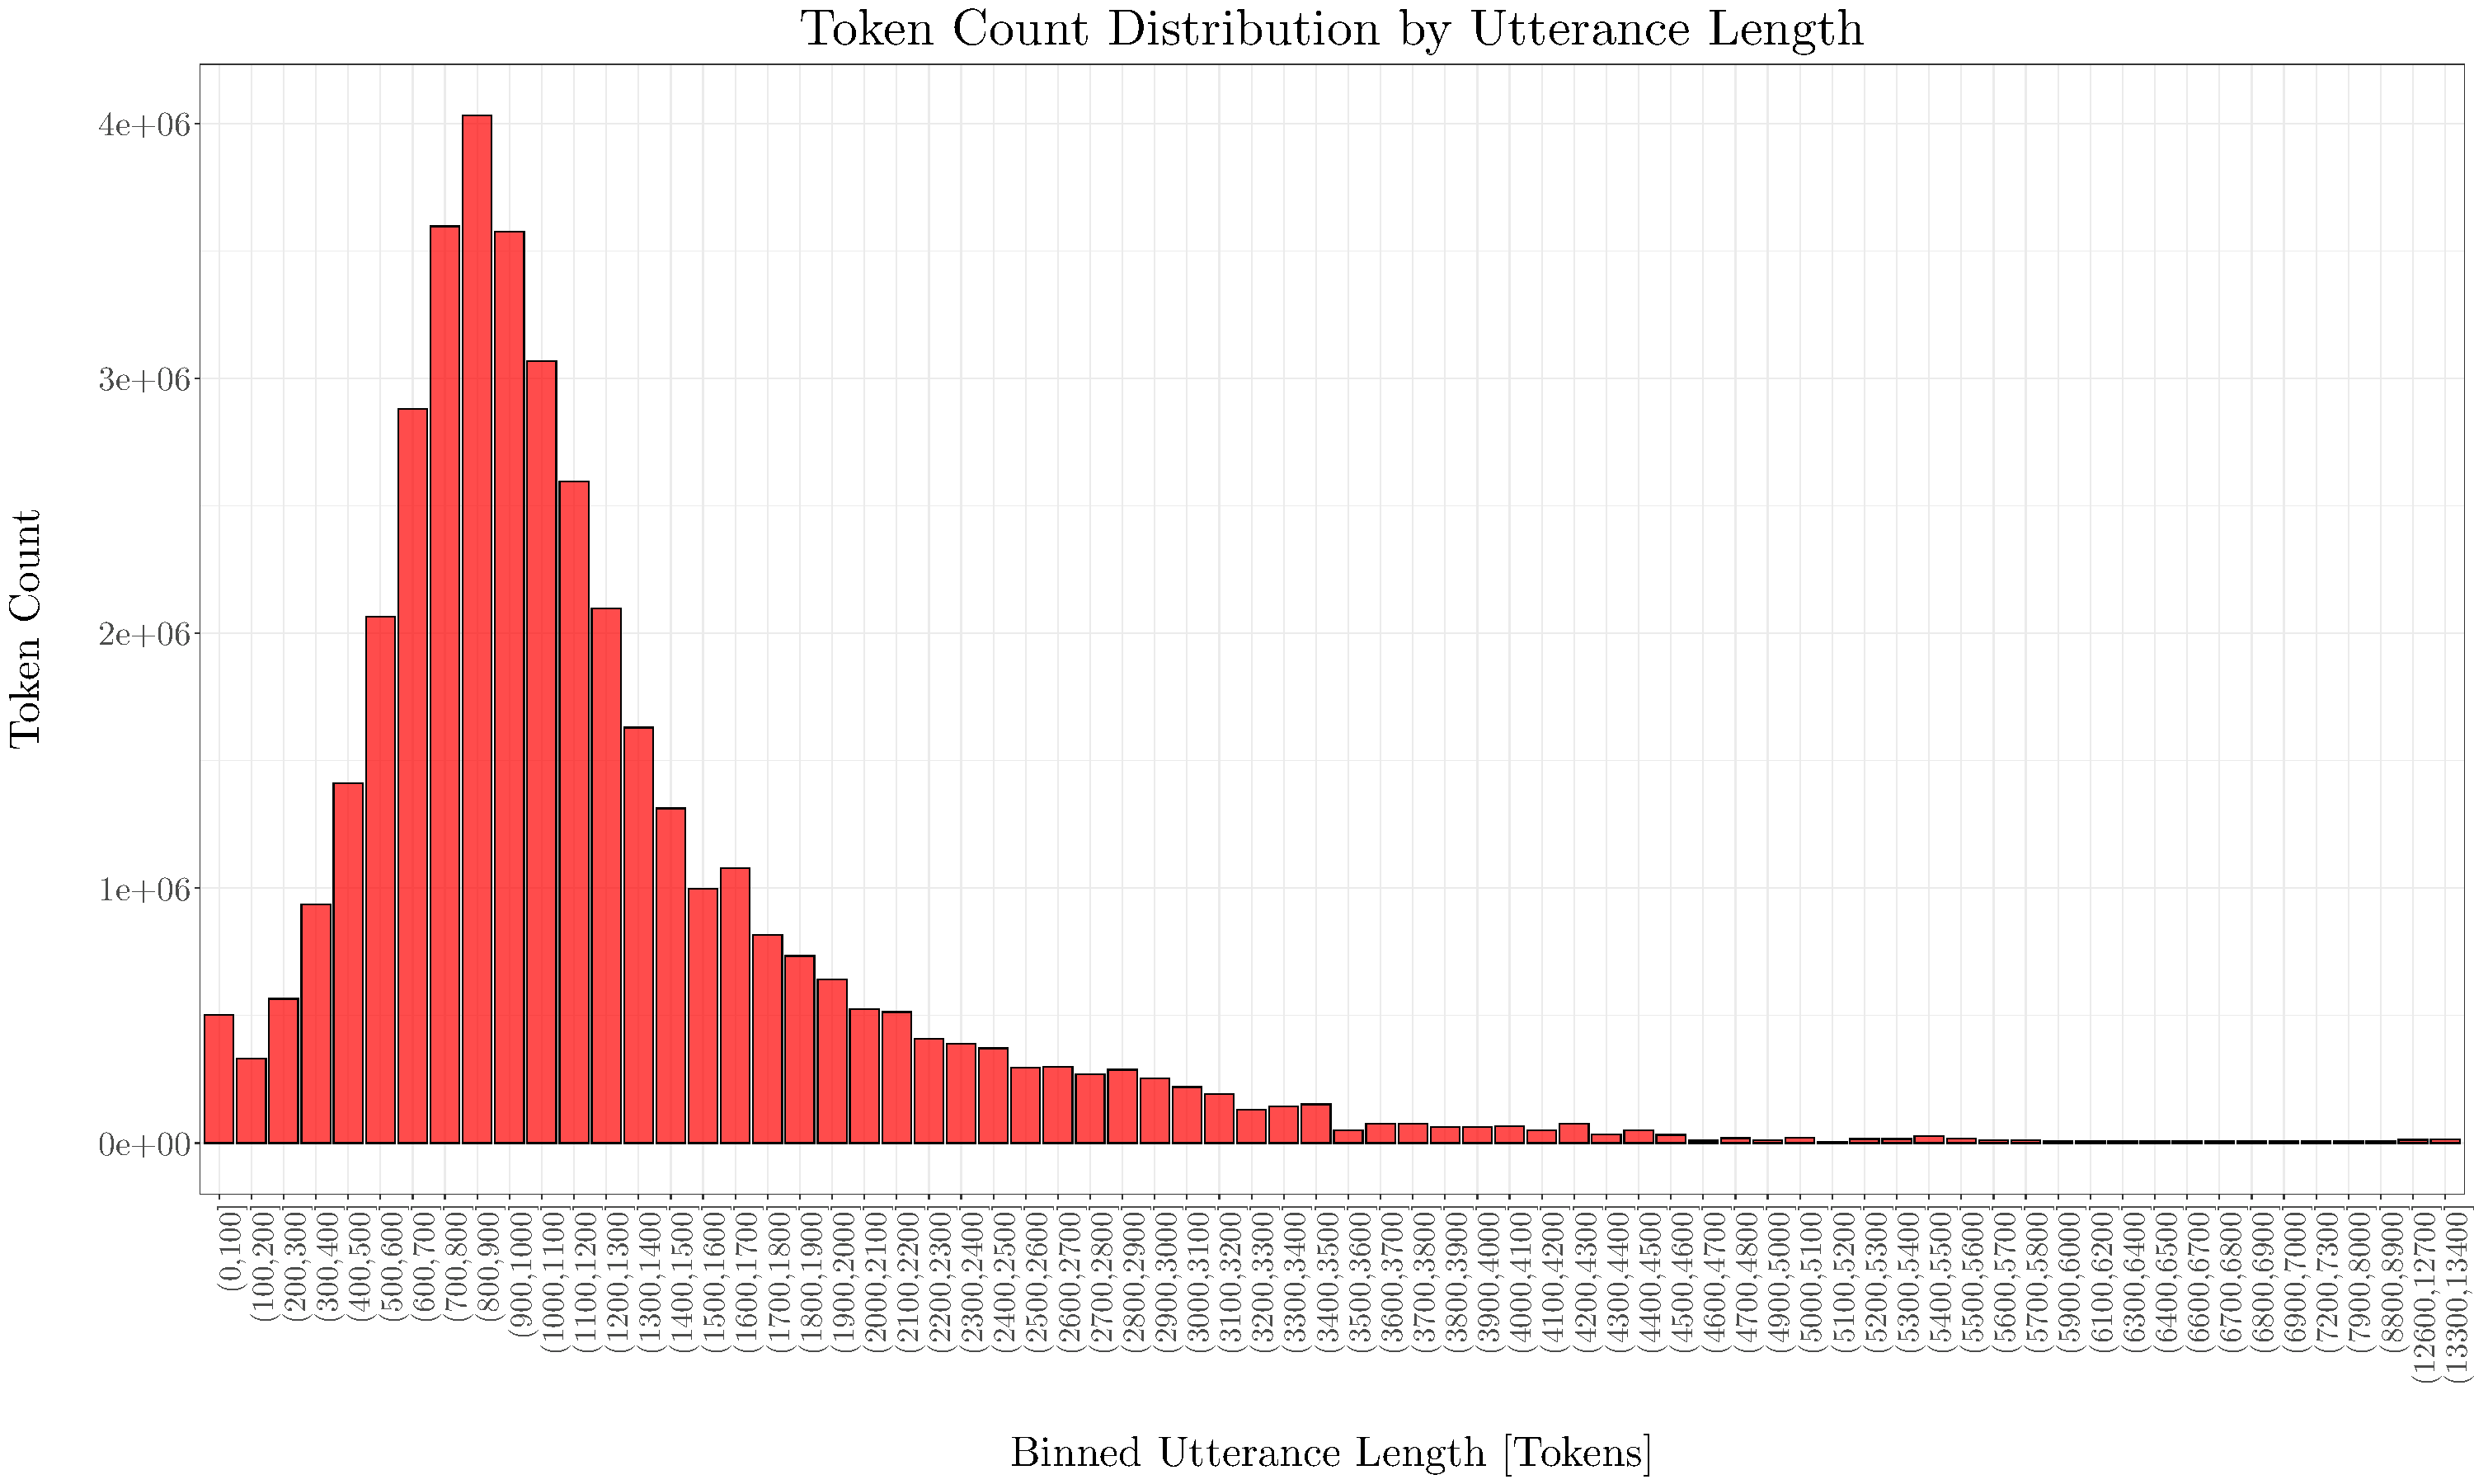
\includegraphics[trim={1.1cm 0.1cm 0 0.1cm},clip,width=\textwidth]{token_dist_UNSC_length.pdf}
    \caption{Token count (top; red) and number of speeches (bottom; blue) by binned speech length in the UNSC corpus}
    \label{UNSC_stats_2}
\end{figure}

To get a better idea of the token statistics of the UNSC speeches, we conducted a simple tokenization and binning procedure on the corpus. Here, we removed certain redundant parts of each speech, such as the initial tokens describing which speaker is speaking. Then we tokenized the left-over speeches using the \texttt{nltk} python module. After this, we binned all of the speeches by their token lengths into intervals of 100 tokens, and plotted the number of tokens and speeches in each binned category as shown in Figure \ref{UNSC_stats_2}.

Here, we can observe that the number of speeches peaks at the binned speech length category of \texttt{(0,100]}, while the number of tokens peaks at the binned speech length category of \texttt{(800,900]} tokens. This tells us that most of the UNSC speeches are generally short and have a length less than or equal to 100 tokens, but the majority of tokens are found in longer length speeches between 800 and 900 tokens. This information will come into further use in later parts of this paper.

\subsection{Sentiment Analysis}

According to \citet{liu2012sentiment}:

\begin{displayquote}
``Sentiment analysis and opinion mining is the field of study that analyzes people's opinions, sentiments, evaluations, attitudes, and emotions from written language. It is one of the most active research areas in natural language processing and is also widely studied in data mining, Web mining, and text mining."
\end{displayquote}

Sentiment analysis can be used to detect various sentiment polarities, for example detecting if a given utterance is positive/negative or subjective/objective \citep{liu2012sentiment}. In such cases, the sentiment value of an utterance typically takes on a real value from --1 to +1, where each extremum indicates one of the polarities of interest. Furthermore, sentiment analysis can be conducted on various granularities or scales \citep{liu2012sentiment}. These can range from a sentence level to a document level and can include various user-defined aspects. For example, given a certain online product review, sentiment analysis could decipher the sentiment polarity towards aspects such as service, product quality and delivery time.

In this paper, we will generally be dealing with sentiment analyses of entire UNSC speeches. This would therefore correspond to sentiment analysis on a document level. In the next subsections, we will proceed to describe some commonly used automatic sentiment analysis tools.

\subsubsection{VADER}

The Valence Aware Dictionary for Sentiment Reasoning (VADER) is a simple rule-based model for general sentiment analysis of social media text \citep{vader}. VADER utilizes a generalized valence-based and human-curated sentiment lexicon to score utterances for their sentiment polarity. Since it was created from handcrafted rules, the VADER sentiment analysis system does not have training data. However, it has been evaluated on various sentiment datasets and shows high classification accuracy; as well as a strong correlation to human-annotator performance \citep{vader}.

VADER has different scoring regimes for sentiment polarities of utterances. Table \ref{table_vader} gives a summary of the various VADER sentiment scores.

\begin{table}[H]
	\centering
	\small
	\setlength{\tabcolsep}{0.5em}
	\def\arraystretch{1.1}
	\begin{threeparttable}
		\begin{tabular}{L{0.2\linewidth} p{0.75\linewidth}}
			\toprule[0.25mm]
			Scores & Description \\
			\midrule[0.35mm]
			\multirow{3}{*}{\shortstack[l]{Positive \\[3pt] Negative \\[3pt] Neutral}}  & All three of these scores refer to the proportion of the input text that is positive, negative or neutral. Ultimately, the sum of the positive, negative and neutral scores must add up to 1. \\[35pt]
			Compound  & The compound score is computed by adding the polarity scores of each word in the sentiment lexicon, adjusted according to the rules, and then normalized between --1 (most extreme negative) and +1 (most extreme positive). One can refer to the compound score as a normalized and weighted composite sentiment score.\\[20pt]
			\bottomrule[0.25mm]
		\end{tabular}
		\caption{Tabular summary of VADER sentiment scores}
		\label{table_vader}
	\end{threeparttable}
\end{table}

One limitation of VADER is that it was constructed to perform on ``microblog-like" contexts found typically on social media platforms such as \textit{Twitter}. However, \citet{vader} do state that VADER is a robust tool and can perform well on diverse domains. For this reason, we consider VADER as a feasible sentiment analysis tool for the UNSC corpus.

\subsubsection{AFINN}
AFINN is a widely used multilingual lexicon containing words and their valence, manually rated between -5 and +5. For sentence-wise rating, the valence of the words is simply aggregated. The latest version of the English AFINN lexicon\footnote{\href{https://github.com/fnielsen/afinn/blob/master/afinn/data/AFINN-en-165.txt}{https://github.com/fnielsen/afinn/blob/master/afinn/data/AFINN-en-165.txt}} contains more than 3,300 words.
The author, Finn Nielsen, has created a Python wrapper called \texttt{afinn} that grants programmers easy access to the lexicon \citep{afinn}.
Despite its simplicity, AFINN performs very well on various tasks in benchmark testing \citep{sentibench}. 
Due to its extensive and relatively unbiased contents, we consider AFINN to be a valuable addition to VADER. The compound scores VADER provides give an idea of the document-level sentiment in the UNSC speeches. For sentence-wise rating, we will rely on AFINN.

\subsubsection{TextBlob}

\texttt{TextBlob} is a python library used for processing textual data. This library also incorporates a successful lexical sentiment analysis tool, which is inherited from the \texttt{pattern} python library. TextBlob's default sentiment analyzer, known as \texttt{PatternAnalyzer}, works in a similar way compared to VADER and assigns sentiment scores to relevant words using a manually annotated sentiment lexicon \citep{smedt2012pattern}. It then averages the lexical sentiment scores to create an overall sentiment score. Table \ref{table_textblob} gives a summary of the two types of scores that this tool can output.

\begin{table}[H]
	\centering
	\small
	\setlength{\tabcolsep}{0.5em}
	\def\arraystretch{1.1}
	\begin{threeparttable}
		\begin{tabular}{L{0.2\linewidth} p{0.75\linewidth}}
			\toprule[0.25mm]
			Scores & Description \\
			\midrule[0.35mm]
			Polarity & This score takes on real-values from --1 to +1, where --1 indicates negative while +1 indicates positive sentiment polarity. \\[20pt]
			Subjectivity  & This score takes on real-values from 0 to +1, where 0 indicates an objective utterance while +1 indicates a subjective utterance.\\[10pt]
			\bottomrule[0.25mm]
		\end{tabular}
		\caption{Tabular summary of TextBlob \texttt{PatternAnalyzer} sentiment scores}
		\label{table_textblob}
	\end{threeparttable}
\end{table}

\subsection{Argumentation Mining}

According to \citet{van2004systematic}:

\begin{displayquote}
``Argumentation is a verbal, social, and rational activity aimed at convincing a reasonable critic of the acceptability of a standpoint by putting forward a constellation of propositions justifying or refuting the proposition expressed in the standpoint."
\end{displayquote}

Argumentation mining can be defined as the process of decomposing text into Argumentative Discourse Units (ADUs) and connecting these units into a comprehensive argumentation tree, where an ADU is defined as the \textit{``span of text that plays a single role for the argument being analyzed, and is demarcated by neighboring text spans that play a different role, or none at all"} \citep{stede2018argumentation}. We will expound further on corpus-specific ADUs and argumentation trees in section \ref{corpora}. \citet{stede2018argumentation} further provide an exhaustive overview for the process of argumentation mining (not necessarily in numerical order):

\begin{enumerate}
    \item Identify argumentative text (or a portion of a text)
    \item Segment the text into ADUs
    \item Identify the central claim
    \item Identify the role/function of ADUs
    \item Identify relations between ADUs
    \item Build the overall structural representation or argumentation tree
    \item Identify the type and the quality of the argumentation
\end{enumerate}

It is worth noting that there exist significant differences in the granularities of ADUs and their corresponding argumentation trees depending on the corpus of reference. Some corpora, such as the argumentative microtext corpus detailed in \citet{peldszus2015annotated}, go into deep detail regarding the relationships between ADUs; specifying central claims, support/attack segments and even describing subtypes of these ADUs, as seen in Figure \ref{args_structure}. Other corpora, such as the US Election Debate corpus detailed in \citet{haddadan-etal-2019-yes}, go into less detail and simply identify ADUs as claims or premises; and only specify basic hierarchies to build an argumentation tree.

Overall, argumentation mining provides the ability to automatically extract important information on the argumentative components of text. This process is extremely valuable for downstream NLP tasks which require distilled information; such as text summarization and question answering.

\begin{figure}[t]
    \centering
    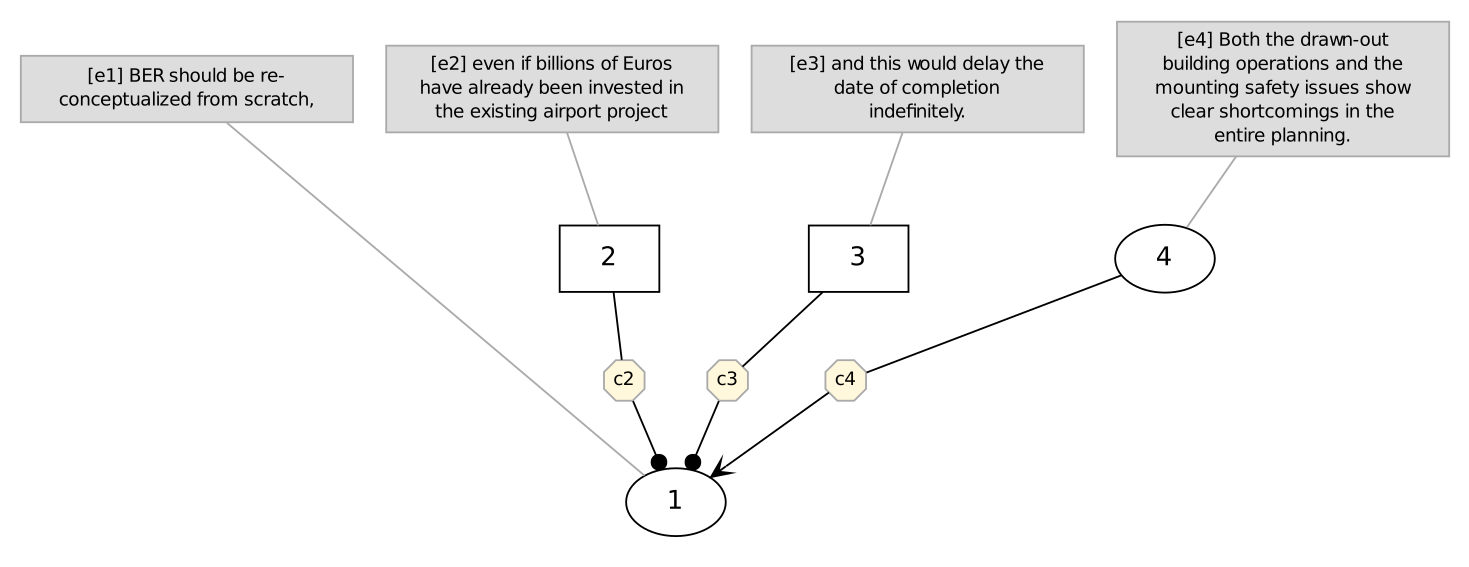
\includegraphics[trim={0cm 0cm 0 0cm},clip,width=\textwidth]{args_structure.png}
    \caption{Sample argumentation tree from argumentative microtext corpus detailed in \citet{peldszus2015annotated}; bottom-most node represents the central claim; arrow-head represents supporting ADU; circle represents attacking ADU}
    \label{args_structure}
\end{figure}

\subsubsection{Copora}
\label{corpora}

As mentioned previously, the granularities of ADUs and the complexity of argumentation trees are usually dependent on the corpus of reference. Table \ref{table_arg_corpora} shows a summary of three high-quality annotated argumentation corpora that are available to the public. Since the ultimate aim of this study is to apply an argumentation classifier on the UNSC corpus, it would make sense to select a well-suited argumentation corpus in order to train a relevant argumentation classifier.

Referring back to Figure \ref{UNSC_stats_2}, we can observe that the UNSC corpus has a wide distribution of speech token lengths. In order to be similar to the UNSC corpus, a well-suited annotated argumentation corpus should have the following properties:

\begin{enumerate}
    \item Relatively long sequence lengths similar to the UNSC corpus; which has a mean sequence length of $\sim$600 tokens.
    \item Sufficiently large number of training data instances with negative (non-argumentative) examples to robustly train an argumentation classifier.
    \item If possible, the corpus should exist in the political domain in order to maximize domain similarity.
    \item If possible, utilize newly published corpus to contribute to research findings.
\end{enumerate}

Given these requirements, points 2, 3, and 4 are satisfied best by the US Election Debate (USED) corpus. Point 1 is best satisfied by the persuasive essay corpus. However, as a mitigating factor towards point 1, the USED corpus has a very large standard deviation to mean ratio in its sequence length; which implies that there are many data instances which are also longer in length.

\begin{table}[t]
	\centering
	\small
	\setlength{\tabcolsep}{0.5em}
	\def\arraystretch{1.1}
	\begin{threeparttable}
		\begin{tabular}{L{0.22\linewidth} L{0.11\linewidth} L{0.17\linewidth} p{0.39\linewidth}}
			\toprule[0.25mm]
			Annotated \qquad Argumentation Corpus & Data \qquad Instances & Seq. Length Statistics \qquad [Tokens]$^{\dagger}$ & \multicolumn{1}
			{L{0.39\linewidth}}{ADU Granularity and \qquad \qquad Argumentation Tree \qquad \qquad Complexity} \\[25pt]
			\midrule[0.35mm]
			Argumentative microtext corpus \citep{peldszus2015annotated} & 
			112 \qquad texts &  $\begin{aligned}[t] % placement: default is "center", options are "top" and "bottom"
\overline{X} &= 78.2\\
\sigma &= 21.5
\end{aligned}$& Fine-grained ADUs with support/attack nature and subtypes, complex argumentation trees \\\\[-5pt]
			Persuasive essay corpus \citep{stab2017parsing} & 402 \qquad \qquad essays & $\begin{aligned}[t] % placement: default is "center", options are "top" and "bottom"
\overline{X} &= 366.0\\
\sigma &= 62.9
\end{aligned}$ & Fine-grained ADUs with support/attack nature, complex argumentation trees \\\\[-5pt]
			US election debate corpus \citep{haddadan-etal-2019-yes} & 6,559 speech turns & $\begin{aligned}[t] % placement: default is "center", options are "top" and "bottom"
\overline{X} &= 110.4\\
\sigma &= 151.6
\end{aligned}$ & Coarse ADUs as either claims or premises, simple argumentation trees \\[25pt]
			\bottomrule[0.25mm]
		\end{tabular}
    \begin{tablenotes}[flushleft]
      \scriptsize
      \item $^{\dagger}\overline{X}$ and $\sigma$ represent the mean and standard deviations of sequence token lengths
    \end{tablenotes}
		\caption{Tabular summary of three prospective annotated argumentation corpora}
		\label{table_arg_corpora}
	\end{threeparttable}
\end{table}

\subsubsection{Models}
\label{models}

In order to gain information about state-of-the-art argumentation classification models, we conducted a survey based on recent publications and summarized key information on three models in Table \ref{table_arg_models}. Since these models were published in or before 2019, we can observe that they were trained/evaluated on the persuasive essay and argumentative microtext corpora, and not the USED corpus due to it only being released in mid-2019.

Furthermore, we can observe that both \citet{potash2016heres} and \cite{kuribayashi2019empirical} train their argumentation classifiers on the assumption that ADU spans in text are pre-defined. This, while being a reasonable assumption for partially annotated text, is not a sound assumption for non-annotated text where there exist no pre-defined ADU spans, as is the case for the UNSC corpus.

This limitation was in fact noted by \citet{eger2017neural}, which perhaps inspired them to create a more ground-up methodology of conducting sequence tagging in order to classify ADU spans, types and linkages altogether as a joint task. This technique of sequence tagging to form a ground-up framework is notable and will be revisited in section \ref{fine_tune} of this study.

Another limitation of all three models is their language encoding techniques. Recent developments in NLP have shown that transformer-based language models, such as BERT, far outperform other language encodings such as Bag-of-Words, GloVe and ELMo \citep{devlin2018bert}. Exploring new BERT-style language encodings could be an interesting avenue to further our research.

\begin{table}[t]
	\centering
	\small
	\setlength{\tabcolsep}{0.5em}
	\def\arraystretch{1.1}
	\begin{threeparttable}
		\begin{tabular}{L{0.19\linewidth} L{0.10\linewidth} L{0.20\linewidth} L{0.17\linewidth} L{0.21\linewidth}}
			\toprule[0.25mm]
			Model & Corpus$^{\dagger}$ & Task & Language \qquad Encoding & Best Performance \qquad [Macro-F$_1$]$^{\ddagger}$ \\
			\midrule[0.35mm]
			Joint Pointer \qquad Network \citep{potash2016heres} & PEC \qquad MTC & Classify ADU types and linkages given pre-defined spans & Bag-of-Words \qquad GloVe & PEC: 0.801 \qquad \qquad MTC: 0.777 \\\\[-5pt]
			BLCC tagger and LSTM-ER \citep{eger2017neural} & PEC & Sequence tagging for ADU spans, types and linkages & GloVe & Exact: 0.449  \qquad Half-span: 0.505 \\\\[-5pt]
			Span-based \qquad BiLSTM \citep{kuribayashi2019empirical} & PEC \qquad MTC & Classify ADU types and linkages given pre-defined spans & GloVe \qquad ELMo & PEC: 0.818 \qquad \qquad MTC: 0.782 \\[20pt]
			\bottomrule[0.25mm]
		\end{tabular}
    \begin{tablenotes}[flushleft]
      \scriptsize
      \item $^{\dagger}$PEC: Persuasive Essay Corpus, MTC: Argumentative Microtext Corpus
      \item $^{\ddagger}$Where necessary, F$_1$ scores were averaged amongst joint tasks for brevity
    \end{tablenotes}
		\caption{Tabular summary of three state-of-the-art argumentation classification models}
		\label{table_arg_models}
	\end{threeparttable}
\end{table}

\subsection{Transformer-Based Language Models}

Since the introduction of the transformer architecture in the iconic ``Attention is all you need" paper by \citet{vaswani2017attention}, we have seen the transformer architecture being used extensively in various NLP tasks, particularly in unsupervised language encoding. Transformers show significant advantages over traditional recurrent encoder-decoder frameworks due to their self-attention mechanism; which has shown to both increase performance, and efficiency through improved parallelization \citep{vaswani2017attention}.

Since previous argumentation models shown in Table \ref{table_arg_models} did not leverage on state-of-the-art transformer architectures, it could be a good addition for us to conduct our research using such transformer architectures.

\subsubsection{BERT}
\label{bert}

BERT, which abbreviates Bidirectional Encoder Representations from Transformers, is a novel context-aware language model trained using transformers \citep{devlin2018bert}. After pre-training on unsupervised language modeling tasks, BERT can be fine-tuned for downstream NLP tasks such as question-answering and natural entity recognition \citep{devlin2018bert}. A schematic for this process can be seen in Figure \ref{bert_schematic}. Fine-tuning BERT on various NLP tasks has shown significant performance improvements over preceding baselines; which is a large factor for recent academic interest and publications regarding the model.

\begin{description}[style=nextline]
\item [Architecture] In \citet{devlin2018bert}, two variants of BERT known as BERT$_{\text{BASE}}$ ($L=12$, $H=768$, $A=12$, $P=110$ million) and BERT$_{\text{LARGE}}$ ($L=24$, $H=1024$, $A=16$, $P=340$ million) were tested; where $L$ refers to the number of transformer blocks, $H$ refers to the hidden size, $A$ refers to the number of self-attention heads and $P$ refers to the total number of parameters. The models were trained on 4 and 16 Cloud TPUs respectively, training for a total of 4 days.

\begin{figure}[t]
    \centering
    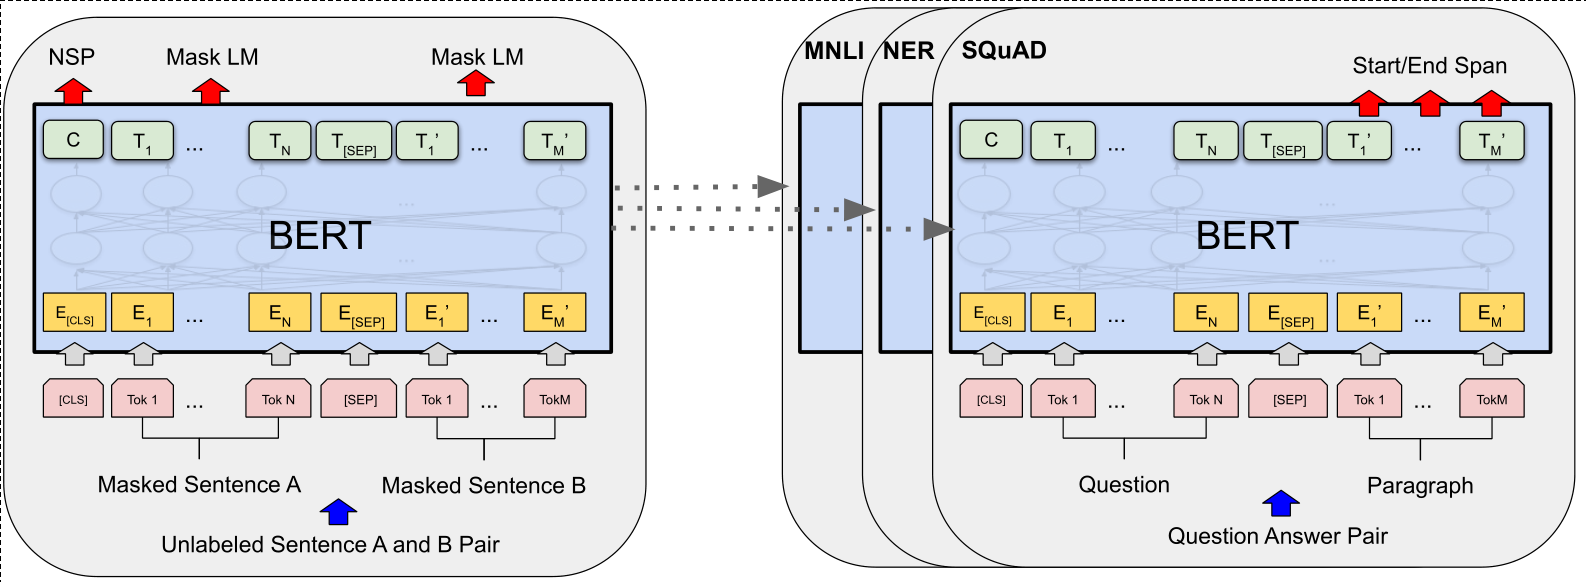
\includegraphics[trim={0.1cm 0cm 0cm 0.1cm},clip,width=\textwidth]{bert_schematic.png}
    \caption{Schematic of BERT pre-training (left) and fine-tuning (right) for downstream NLP tasks \citep{devlin2018bert}}
    \label{bert_schematic}
\end{figure}

\item [Pre-training Tasks] BERT was trained with two pre-training objectives; namely Masked Language Model (MLM) and Next Sentence Prediction (NSP). Under the MLM task, some percentage of input tokens are masked at random and the model is trained to predict the identities of the masked tokens. This task incorporates a global context of the input text, since all of the context would be necessary to predict the masked token(s). Under NSP, some consecutive sentences are shuffled at random and BERT learns to predict whether sentence B indeed follows sentence A. Through this process, BERT incorporates sequential context for natural language understanding and this pre-training task has been shown to help with downstream NLP tasks such as question-answering.

\item [Special Tokens] BERT incorporates certain special tokens in order to perform the aforementioned pre-training tasks; namely \texttt{[CLS]}, \texttt{[SEP]}, \texttt{<pad>} and \texttt{<unk>}. The \texttt{[CLS]} token is found at the start of every sequence and its position in the model output represents the aggregate representation of the entire sequence; which is why this token's position is used for sequence classification tasks. The \texttt{[SEP]} token is a separator token which is used to separate sentence pairs for the NSP pre-training task. \citet{devlin2018bert} also suggests that the \texttt{[SEP]} token should be used at the end of sequences; although there are some discrepancies regarding this in their paper. For simplicity, we assume that the \texttt{[SEP]} token should additionally be placed at the end of input sequences. The \texttt{<pad>} and \texttt{<unk>} tokens represent padding and unknown tokens respectively. BERT additionally enforces a maximum input sequence length of 512 tokens.

\item [WordPiece Tokenization] BERT uses the WordPiece Model (WPM) for tokenization of its input text. The WPM is a novel and powerful tokenization model that tokenizes words into sub-word units \citep{wu2016google}. This is a powerful approach as it mitigates the large vocabularies and out-of-vocabulary (OOV) issues of purely word-based tokenizers, as well as the small vocabularies and semantic information loss of purely character-based tokenizers. Following is an example of the WPM model's output, which has been adapted from \citet{wu2016google}:

\begin{description}
    \item [Input Sequence:] Jet makers feud over seat widths
    \item [WordPiece Output:] $\_$J et $\_$makers $\_$fe ud $\_$over $\_$seat $\_$width s
\end{description}

``$\_$" is a special character used to mark the beginning of a word. A token which does not start with ``$\_$" is a segmented sub-word of a main word; for example ``et" being a sub-word of ``Jet" in the example above. It is worth noting here that a combination of using the WPM and special tokens in BERT result in input sequences becoming much longer than they originally were. As a result, some input sequences in corpora might exceed BERT's 512 token hard upper-limit and might need to be discarded from analysis.

\item [Fine-tuning] For pre-training BERT, large unsupervised corpora such as BookCorpus (800 million words) and English Wikipedia (2,500 million words) are used \citep{devlin2018bert}. Fine-tuning follows after pre-training and involves slightly adjusting all the parameters in BERT in order to perform on downstream NLP tasks and corresponding supervised corpora. Compared to pre-training, fine-tuning is relatively fast and computationally inexpensive \citep{devlin2018bert}. Fine-tuning BERT on downstream NLP tasks has shown significant improvements in state-of-the-art performances, which include a 7.7$\%$ point absolute improvement of the GLUE score for the General Language Understanding Evaluation (GLUE) task.
\end{description}

\subsubsection{ALBERT}
\label{albert}

\begin{figure}[t]
    \centering
    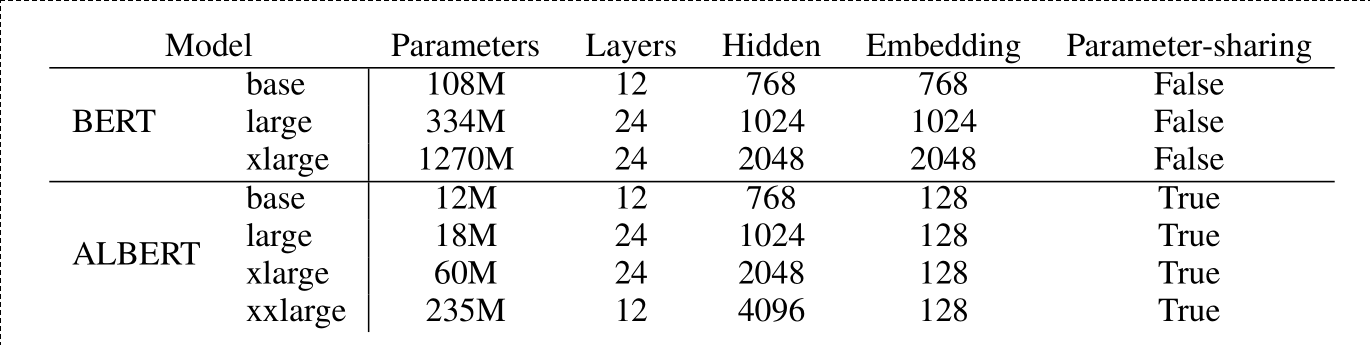
\includegraphics[trim={0.2cm 0cm 0cm 0.2cm},clip,width=\textwidth]{img/albert_comparison.png}
    \caption{Tabular excerpt from \citet{lan2019albert} on BERT vs. ALBERT architecture}
    \label{albert_comparison}
\end{figure}

A major criticism of the aforementioned BERT language model is its sheer size in terms of parameters; which can ultimately lead to GPU/TPU memory limitations, long training times and unexpected model degradation. To address these issues, \citet{lan2019albert} propose a ``lite" version of BERT (a.k.a. ALBERT) which utilizes factorized embedding parameterization and cross-layer parameter sharing to reduce memory consumption and increase training speed. Figure \ref{albert_comparison} shows how this optimization results in a drop in the number of parameters in the ALBERT model(s); for example the ALBERT$_{\text{BASE}}$ model can be reduced to 12 million parameters, making it a suitable candidate to train even on a single GPU.

To further improve performance, \citet{lan2019albert} replace the NSP task in BERT's unsupervised pre-training with a sentence-order prediction (SOP) task. This involves the same task as per NSP for positive examples. However, negative examples involve two consecutive sentences being swapped in terms of their order. According to \citet{lan2019albert}, the SOP task pushes ALBERT to learn more fine-grained distinctions on discourse-level coherence properties. This modification has shown to improve downstream NLP task performance for multi-sentence problems. Additionally, ALBERT uses the SentencePiece tokenization model (SPM) from \citet{kudo2018sentencepiece}, which incorporates the Unigram Language Model (ULM) from \citet{kudo2018subword}. The SPM is similar to BERT's WPM, but is purportedly faster and more versatile compared to the WPM.

Despite these key differences, ALBERT is still very similar to BERT in terms of its general architecture and building blocks, which can be seen as well in Figure \ref{albert_comparison}. Additionally, it is worth noting that the 512 token hard upper-limit for input sequences also applies for ALBERT. Ultimately, since ALBERT has shown to both perform and scale better than its BERT counterpart (with particular focus on discourse-level coherence for its SOP task), we consider ALBERT as a viable model for use in our argumentation mining task. This application will be further expounded on in section \ref{fine_tune} of our study.